\chapter{Validation}

Here we present a series of reproduced results from the scientific literature as 
a validation of our computational implementation. We manage to reproduce the 
instantaneous dipole results from the simulation of the 
hydrogen molecule in \citeauthor{li2005time}\cite{li2005time},
the time-dependent ground state probability of a quantum dot from 
\citeauthor{Zanghellini04}\cite{Zanghellini04}
and the spectrum of Helium from
\citeauthor{pedersen2019symplectic}\cite{pedersen2019symplectic}.
The simulation of the ionisation of beryllium 
from \citeauthor{miyagi2013time}\cite{miyagi2013time},
serves as an illustration of the advantage of
adaptive orbitals versus static orbitals in a time-dependent coupled cluster method.
For all time-dependent studies in this chapter we have employed the symplectic 
\lstinline{GaussIntegrator} integrator class, as it has shown to be most stable in 
preliminary studies.


\section{Instantaneous dipole in $H_2$}

\citeauthor{li2005time}\cite{li2005time} employ a time-dependent Hartree-Fock 
apporach in order to study the electronic optical response of molecules 
in intense fields. To be specific, they model the hydrogen molecule $H_2$ 
with a \lstinline{6-311++G(d,p)} basis set, subject to an oscillating field 
of $1.72\times10^{13}\text{ W} \text{cm}^{-2}$ and $456\text{ nm}$. They find the time-dependent
Hartree-Fock method to be nearly indistinguishable from calculations using the 
full time-dependent Schrödinger equation. We have managed to replicate the 
instantaneous dipole of this simulation of hydrogen.

A \lstinline{6-311++G(d,p)} basis set corresponds to a \lstinline{6-311++Gss} 
basis set in \lstinline{PySCF}, and we can extract it from here,
\begin{python}
molecule = "
    h 0.0 0.0 -0.6948522960236121;
    h 0.0 0.0  0.6948522960236121
    "
basis = "6-311++Gss"
system = construct_pyscf_system_ao(molecule, basis=basis)
\end{python}
The bond length of the Hydrogen molecule is approximately $0.7354\text{ Å}$, converted 
to multiples of Bohr radii here. As the naming suggests, the basis set is a split-valence 
triple-zeta basis set, with one added s-type diffuse function and a set of p-type
polarisation 
functions for each Hydrogen atom\footnote{This would be obvious for a quantum chemist,
but basis set configurations looks like incantantions from a spellbook to the 
uninitiated physicist}.

In their simulations \citeauthor{li2005time} have used a linearly polarised and 
spatially homogenous external field aligned along the $z$-axis, 
\begin{equation}
    \vb{e}(t) = \vb{E}(t)\sin(\omega t).
\end{equation}
The field envelope $|\vb{E}|$ is linearly increased with time to a maximum value 
$|\vb{E}_\text{max}|$ at the end of the first cycle and remains at $|\vb{E}_\text{max}|$
for one cycle and then decreases linearly to zero by the end of the next cycle,
\begin{equation}
    \label{eq:li_laser}
    \begin{aligned}
        \vb{E}(t) = (\omega t / 2\pi) \vb{E}_\text{max} \quad &\text{for} \quad
            0 \leq t \leq 2\pi / \omega \\ 
        \vb{E}(t) = \vb{E}_\text{max} \quad &\text{for} \quad 
            2\pi / \omega \leq t \leq 4\pi / \omega \\ 
        \vb{E}(t) = (3 - \omega t / 2\pi) \vb{E}_\text{max} \quad &\text{for} \quad 
            4\pi / \omega \leq t \leq 6\pi / \omega \\
        \vb{E}(t) = 0 \quad &\text{for} \quad
            t < 0 \text{ and } t > 6\pi / \omega,
    \end{aligned}
\end{equation}
where the maximum field intensity if $1.72\times10^{14} \text{ W} \text{cm}^{-2}$ 
($E_\text{max} = 0.07 \text{ au}$). \citeauthor{li2005time} also run a simulation 
for a lower intensity, but we are conecerned only with this relatively more intensive 
pulse. The entire simulation lasts for $T=225 \text{ au}$.

The result of our simulation is shown in \autoref{fig:li_compare}, where we have 
computed the instantaneous dipole over time using three different methods. The 
time-dependent Hartre-Fock result is shown in the bottom sub-figure, and is expected 
to be exactly the same as figure 4.a from \citeauthor{li2005time}\cite{li2005time},
which it appear to be. For comparrison we have computed the result with both of 
our time-dependent coupled cluster methods. The result of the time-dependent 
coupled cluster method with single and double excitations are showed in the top subfigure,
and the result of the orbital-adaptive coupled cluster method with double excitations 
are shown in the middle subfigure. We see that there is no perceptible difference between 
the results of the three methods.

\begin{figure}
    \centering
    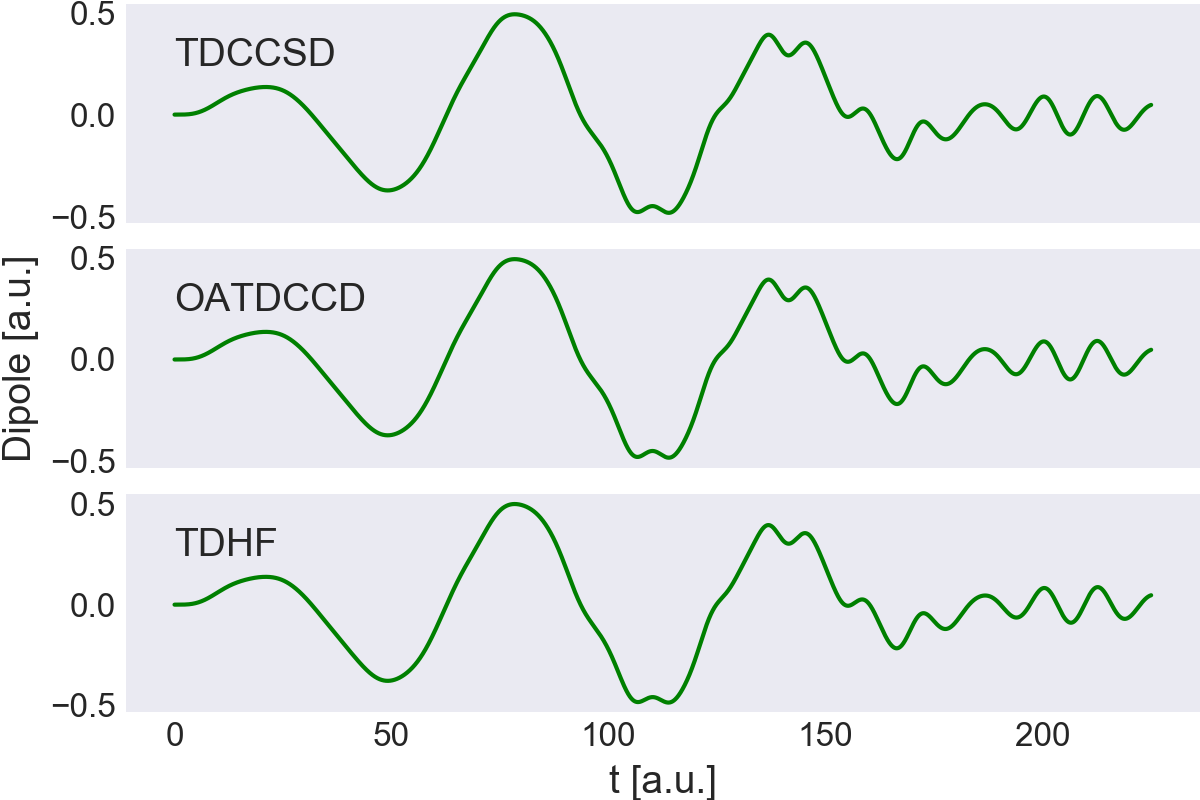
\includegraphics[width=0.75\textwidth]{results/figures/li_compare.png}
    \caption{Instantaneous dipole for $H_2$ in an oscillating electric field
        $E_\text{max} = 0.07 \text{ au}$ ($1.72\times10^14 \text{ W} \text{cm}^{-2}$)
        and $\omega=0.1 \text{ au}$ ($456\text{ nm}$) using a \lstinline{6-311++G(d,p)}
        basis set.
    }
    \label{fig:li_compare}
\end{figure}


\section{Ground State Probability in 1D Quantum Dot}

\citeauthor{Zanghellini04}\cite{Zanghellini04} calculate the time development of a 
one-dimensional quantum dot with two electrons using the multi-configurational 
time-dependent Hartree-Fock method (MCTDHF). This method yields excact results for 
a very large number of configurations, $\eta \to \infty$. This study would provide a 
proper benchmark for our implementation because the coupled cluster method with singles and 
doubles excitations (CCSD) is excact for $n=2$ particles. 
The harmonic oscillator potential applied in
their study had a frequency of $\Omega=0.25$, used a strong laser-like field with 
maximum intensity of $\vb{E} = 1$ and a laser frequency of $\omega = 8 \Omega = 2$.
The oscillating field is described much more simply than in
\citeauthor{li2005time}\cite{li2005time}, using a simple sine function,
\begin{equation}
    \vb{e}(t) = \vb{E}\sin(\omega t),
\end{equation}
where the envelope $\vb{E}$ does not vary in time.

\citeauthor{Zanghellini04}\cite{Zanghellini04} find that their multi-configurational time-dependent
Hartree-Fock scheme convergences as the number of configurations is 
$\eta \geq15$, up to the resulotion of their figures.
We are able to reproduce this result precisesly by employing the 
time-dependent coupled cluster method with singles and double excitations (TDCCSD).
We have used our own one-dimensional quantum dot class, \lstinline{ODQD}, with 
a harmonic potential and $l=20$ spin-orbitals
in the basis set for this simulation.

\begin{figure}
    \centering
    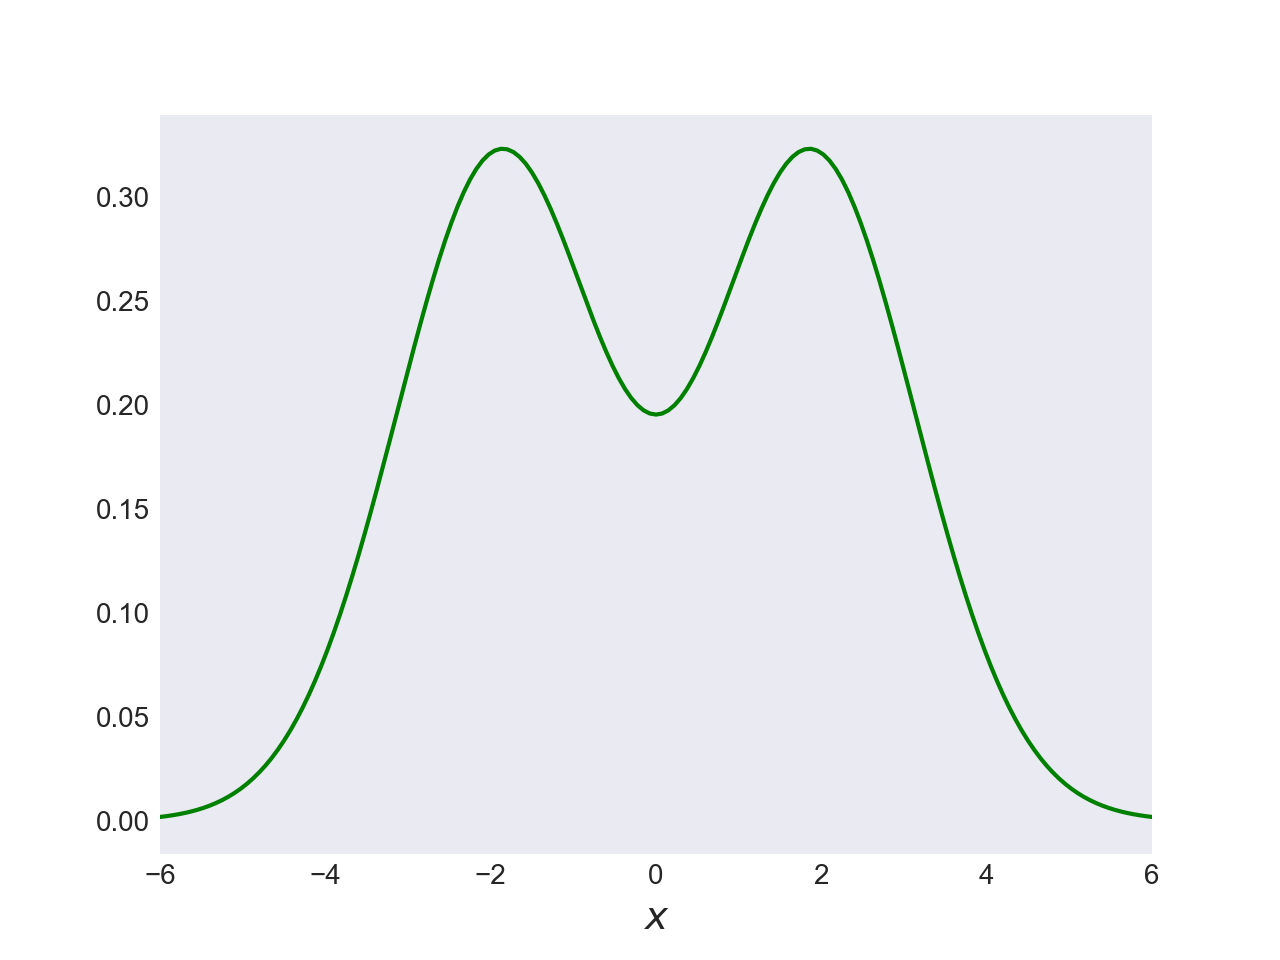
\includegraphics[width=0.75\textwidth]{results/figures/zanghellini_fig1.png}
    \caption{
        \label{fig:zanghellini_fig1}
        Electron density for the ground state wavefunction of a quantum dot with 
        $n=2$ eletrons and $l=20$ spin-orbitals in the basis set computed with
        CCSD. This plot 
        corresponds precisely with figure 1 in
        \citeauthor{Zanghellini04}\cite{Zanghellini04}.
    }
\end{figure}

\begin{figure}
    \centering
    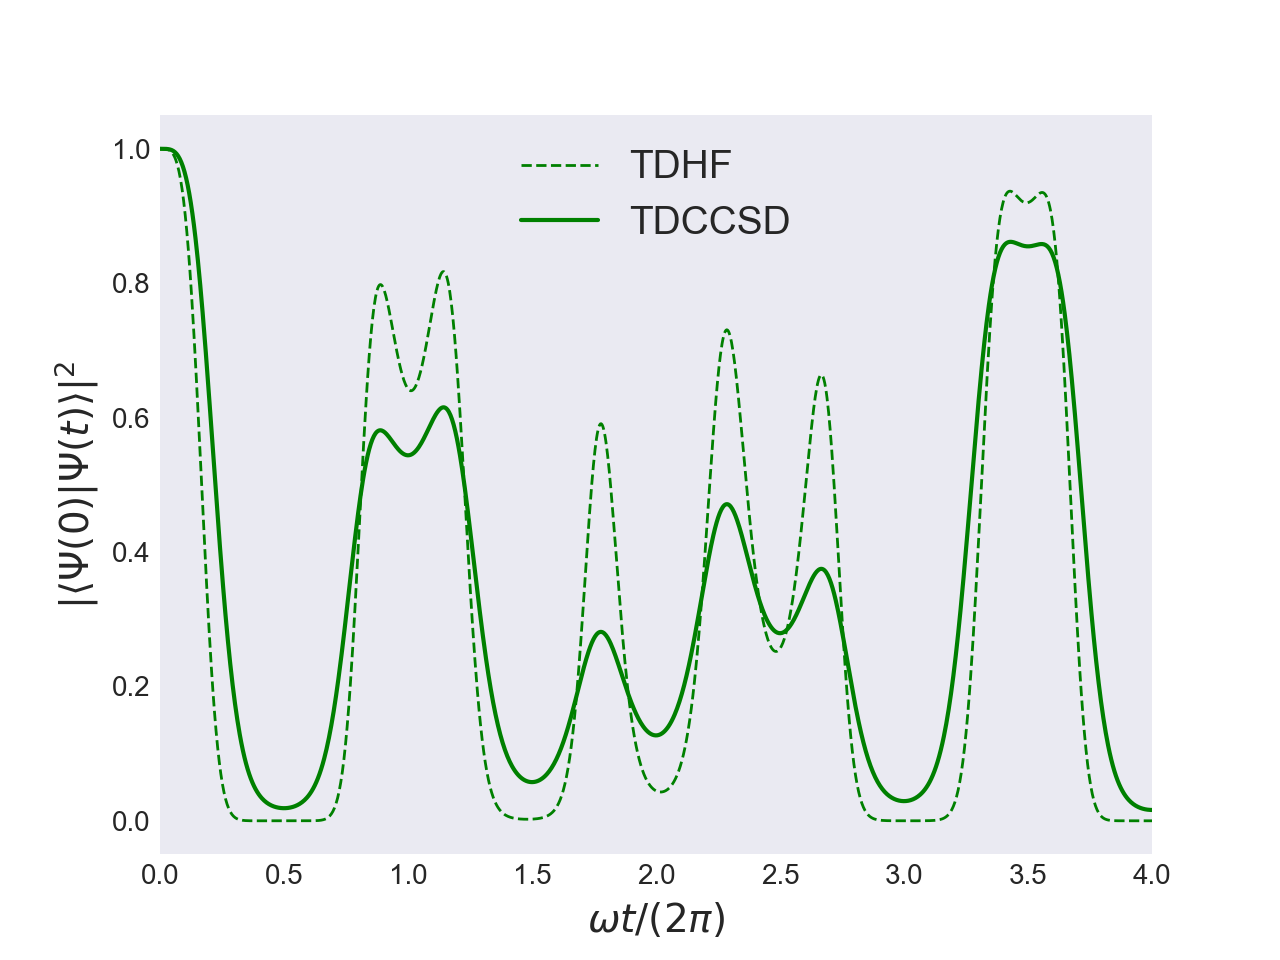
\includegraphics[width=0.75\textwidth]{results/figures/zanghellini_fig2.png}
    \caption{
        \label{fig:zanghellini_fig2}
        Probability of being in the ground state $|\braket{\Psi(0)}{\Psi(t)}|$
        using both TDHF and TDCCSD, for a one-dimensional quantum dot with $n=2$
        particles and $l=20$ spin-orbitals. This plot corresponds precisely with 
        figure 2 in \citeauthor{Zanghellini04}\cite{Zanghellini04}.
    }           
\end{figure}

In \autoref{fig:zanghellini_fig1} we see the ground state electron density for the 
ground state wavefunction computed with CCSD. \citeauthor{Zanghellini04} computed the electron
density for an increasing number of configurations $\eta$ using multi-configurational
time-dependent Hartree-Fock (MCTDHF). This figure matches the convergent electron density found by
\citeauthor{Zanghellini04} as $\eta \to \infty$, in figure 1 from their article. 

\autoref{fig:zanghellini_fig2} depicts the probability for the system being in the ground 
state as a function of time. Here we have included both a time-dependent Hartree-Fock
computation, corresponding to a multi-configurational time-dependent 
Hartree-Focke computation with $\eta=1$ configurations, and 
a time-depenedent coupled cluster computation with single and double excitations.
We see that our coupled cluster scheme corresponds to the multi-configurational Hartree-Fock 
scheme employed by \citeauthor{Zanghellini04} when $\eta\to\infty$, as
\autoref{fig:zanghellini_fig2} match figure 2 in
\citeauthor{Zanghellini04}\cite{Zanghellini04} precisely.


\section{Dipole Spectrum of Helium}

In their comparison study of symplectic and regular Runge-Kutta type integrators, 
\citeauthor{pedersen2019symplectic}\cite{pedersen2019symplectic} produce a dipole 
spectrum of helium. 

The basis set employed by \citeauthor{pedersen2019symplectic} is a cc-pVDZ 
basis set which we extract from \lstinline{Psi4},
\begin{python}
He = "
    He 0.0 0.0 0.0
    symmetry c1
"
options = {"basis": "cc-pvdz", "scf_type": "pk", "e_convergence": 1e-8}
system = construct_psi4_system(He, options)
\end{python}
The \lstinline{cc-pVDZ} basis set is a correlation consistent, polarised, valence-only 
basis set with double zeta-functions. For hydrogen this basis set amounts to five 
orbitals in total.

% \omega=2.8735643 \text{ au}
In their study \citeauthor{pedersen2019symplectic} use an oscillating field with 
frequency $\omega=2.8736 \text{ au}$ and maximum intensity
$\vb{E}_\text{max} = 10 \text{ au}$. This frequency corresponds to the lowest-lying 
electric-dipole allowed transition from the ground state of helium. The oscillating 
field can be described as 
\begin{equation}
    \vb{e}(t) = \vb{E}(t) \cos(\omega t),
\end{equation}
with a sinusoidal envelope
\begin{equation}
    \label{eq:pedersen_2019_envelope}
    \vb{E}(t) = \vb{E}_\text{max}\sin^2\left(\frac{\pi t}{t_d}\right) H(t_d - t),
\end{equation}
where $H$ is the Heaviside step function designed to return zero when the field 
has reached its designated halting time $t_d$. This envelope is similar in behaviour 
to the one in the study by \citeauthor{li2005time}\cite{li2005time} - it 
increaes gradually at first, and then gradually decreases. 

The oscillating field is only meant to ``disturb'' the ground state of the atom,
as it is quickly 
switched off at $t_d=5$. Then the system is allowed to propagate in time for 
a long period. In our reproduction of the system, we have let the system 
evolve for a total time $T=1500 \text{ au}$. For each time step we compute the 
dipole in the same direction as the polarisation of the oscillating field. The 
fourier transform of this signal will then yield the dipole spectrum of the 
atom. The time-development is performed with the orbital-adaptive time-dependent 
coupled cluster method with double excitations. The result from this simulation is 
depicted in \autoref{fig:helium_spectrum}, which is qualitatively equal to figure 
7 in \citeauthor{pedersen2019symplectic}\cite{pedersen2019symplectic}.

\begin{figure}
    \centering
    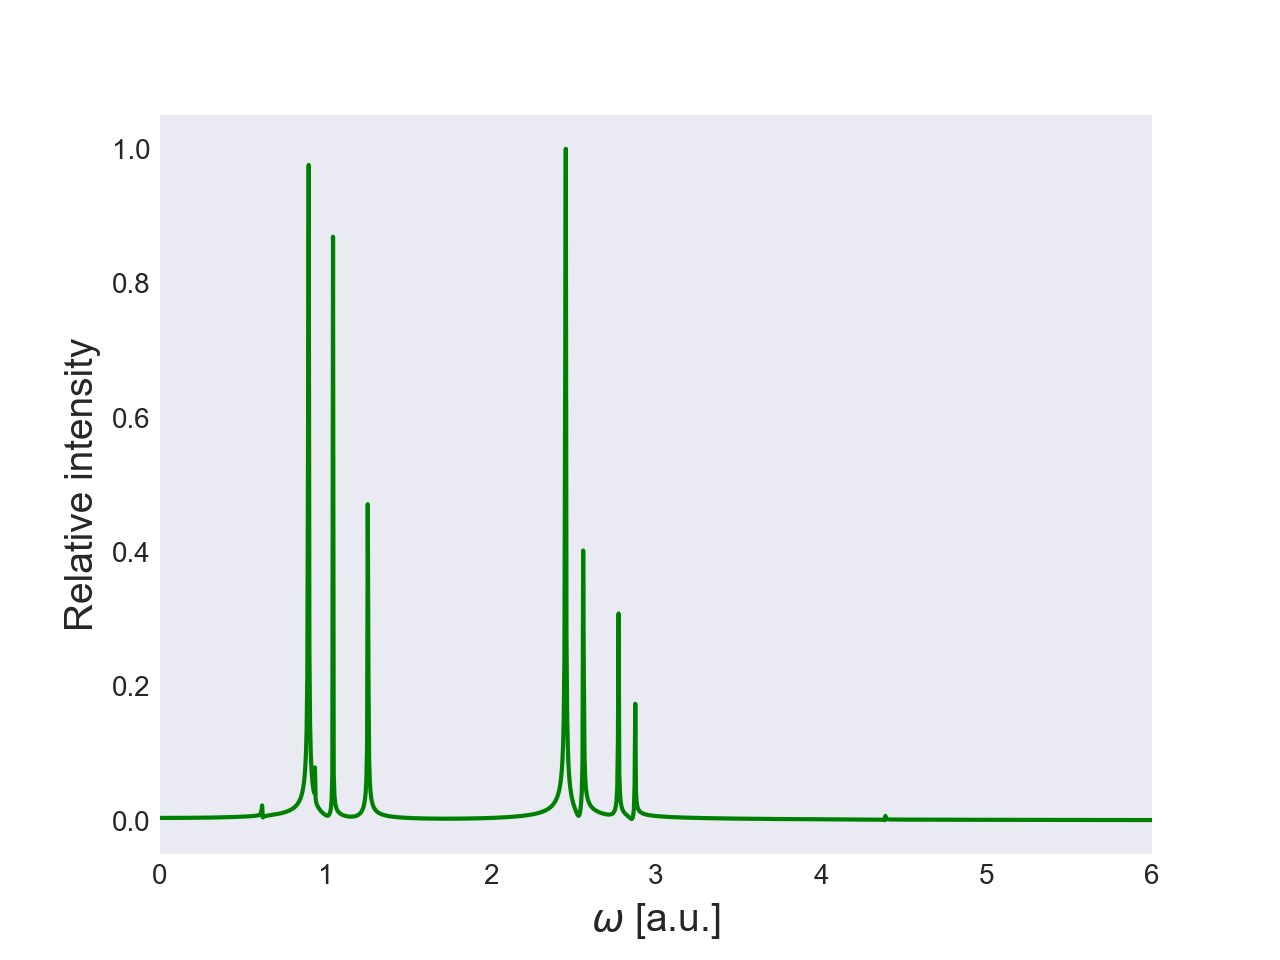
\includegraphics[width=0.75\textwidth]{results/figures/helium_spectrum.png} 
    \caption{Dipole spectrum of He at field strength $10\text{ au}$ using 
        OATDCCD and a \lstinline{cc-pVDZ} basis set.      
    }
    \label{fig:helium_spectrum}
\end{figure}


\section{Ionisation of 1D Beryllium}
\label{sec:miyagi_replication}

\citeauthor{miyagi2013time}\cite{miyagi2013time} implement the time-dependent 
restricted active space self consistent field singles (TD-RASSCF-S) method 
and compare it with time-dependent configuration interaction singles (TDCIS) and 
the multi-configurational time-dependent Hartree-Fock (MCTDHF) method. A simulation they 
perform in this study is the simulation of the ionisation of beryllium. This 
simulation is performed by applying an oscillating field defined by the following 
vector potential,
\begin{equation}
    \vb{A}(t) = \frac{\vb{E}_\text{max}}{\omega}\sin\left(\frac{\pi t}{T} \right),
\end{equation}
giving the following field
\begin{equation}
    \vb{e}(t) = - \vb{E}_\text{max}\sin\left(\frac{\pi t}{T} \right)
    \left[
        \frac{2\pi}{T\omega} \cos\left(\frac{\pi t}{T} \right) \sin\left(\omega t \right)
        + \sin\left(\frac{\pi t}{T} \right) \cos(\omega t)
    \right].
\end{equation}
We reproduce the one-dimensional beryllium model with our \lstinline{AtomicPotential}
class, which can be passed as a potential to the \lstinline{ODQD}
(one-dimensional quantum dot) class when setting up the system,
\begin{python}
Z = 4; n = 4; l = 40; c = 1; a = 1; alpha = 1;
potential = AtomicPotential(Z, c)
odbe = ODQD(n, l, grid_length, num_grid_points, a, alpha)
odbe.setup_system(potential=potential)
\end{python}
where \lstinline{Z} are the number of protons, \lstinline{n} is the number of electrons,
\lstinline{l} is the number of spinorbitals, \lstinline{c} is the position of the nucleus,
\lstinline{a} is the Coulomb screening parameter and \lstinline{alpha} is the strength of the 
Coulomb interaction. We pick a wide grid of $300 \text{ au}$, with $5001$ points, and 
a time step size of $dt=0.01$.

The idea behind the simulation is to compute the particle density over time, and see if 
there is more than significantly high probability to see an electron very far away from the 
nucleus. The total time of the simulation is $T=331 \text{ au}$, and the particle density 
$\rho(x, t)$ is computed at the very beginning of the simulation, halfway through 
and at the end of the simulation. We do this both with our time-dependent coupled 
cluster singles doubles (TDCCSD) method with static orbitials and 
the orbital-adaptive time-dependent 
coupled cluster doubles method (OATDCCD). 
The results of the simulations are shown in 
\autoref{fig:miyagi_fig4}.

\begin{figure}
    \centering
    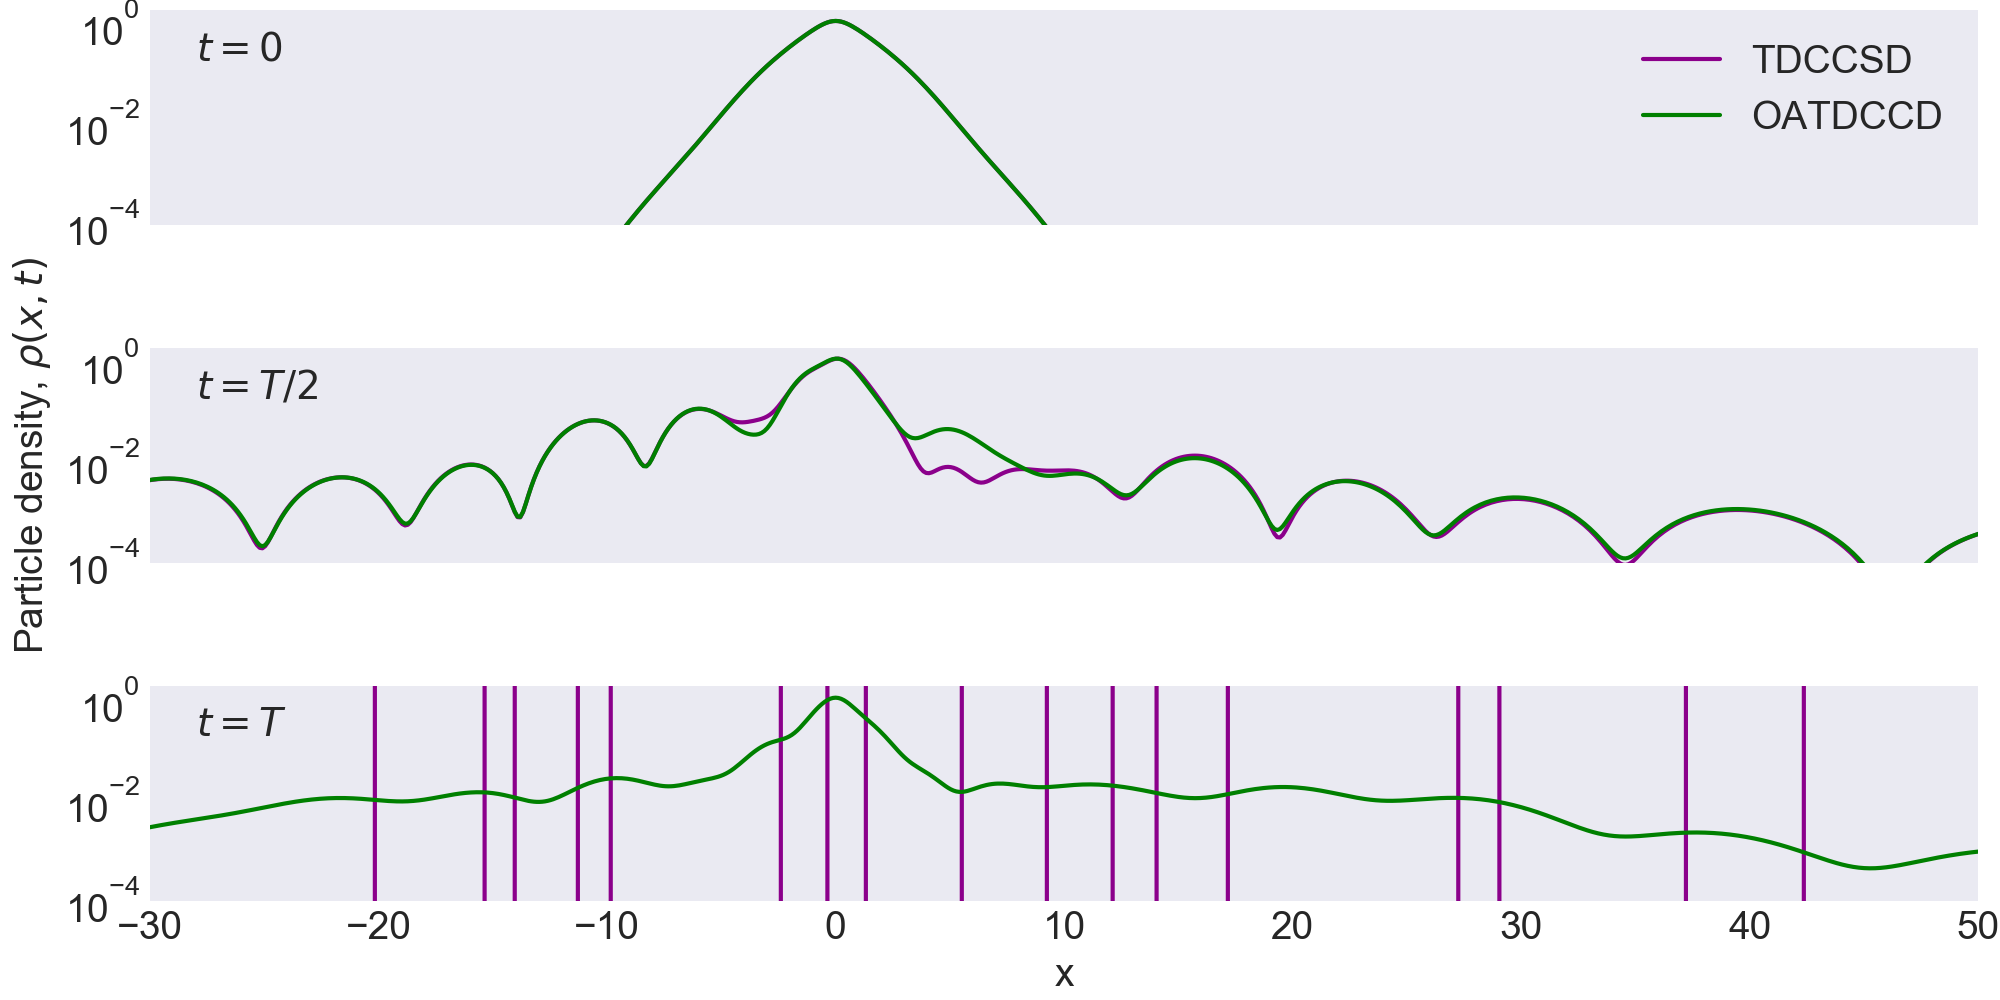
\includegraphics[width=\textwidth]{results/figures/miyagi/fig4_miqyagi.png} 
    \caption{Snapshots of the electron density $\rho(x, t)$ in the 1D beryllium atom 
        at $t=0$, $t=T/2$ and $T$, computed with TDCCSD and OATDCCD. 
    }
    \label{fig:miyagi_fig4}
\end{figure}

In the top subfigure in \autoref{fig:miyagi_fig4} we see the electron density before 
the system is developed in time, and the two methods are in good agreement. In 
the middle subfigure the simulation is halfway through its course and the two methods
both appear to show the same effects, but with 
slight discrepancies. In the bottom subfigure, we see that the OATDCCD method is doing
fine, but the TDCCSD is absolutely non-sensible. We can conclude that the propagating 
obitals in time enables us to get the same qualitative result as \citeauthor{miyagi2013time}
in figure 4 from their study. Keeping the orbitals static as in the TDCCSD method makes 
us unable to model the same behaviour. We will delve a bit deeper to try to shed 
some light on why the TDCCSD method fails.

\begin{figure}
    \centering
    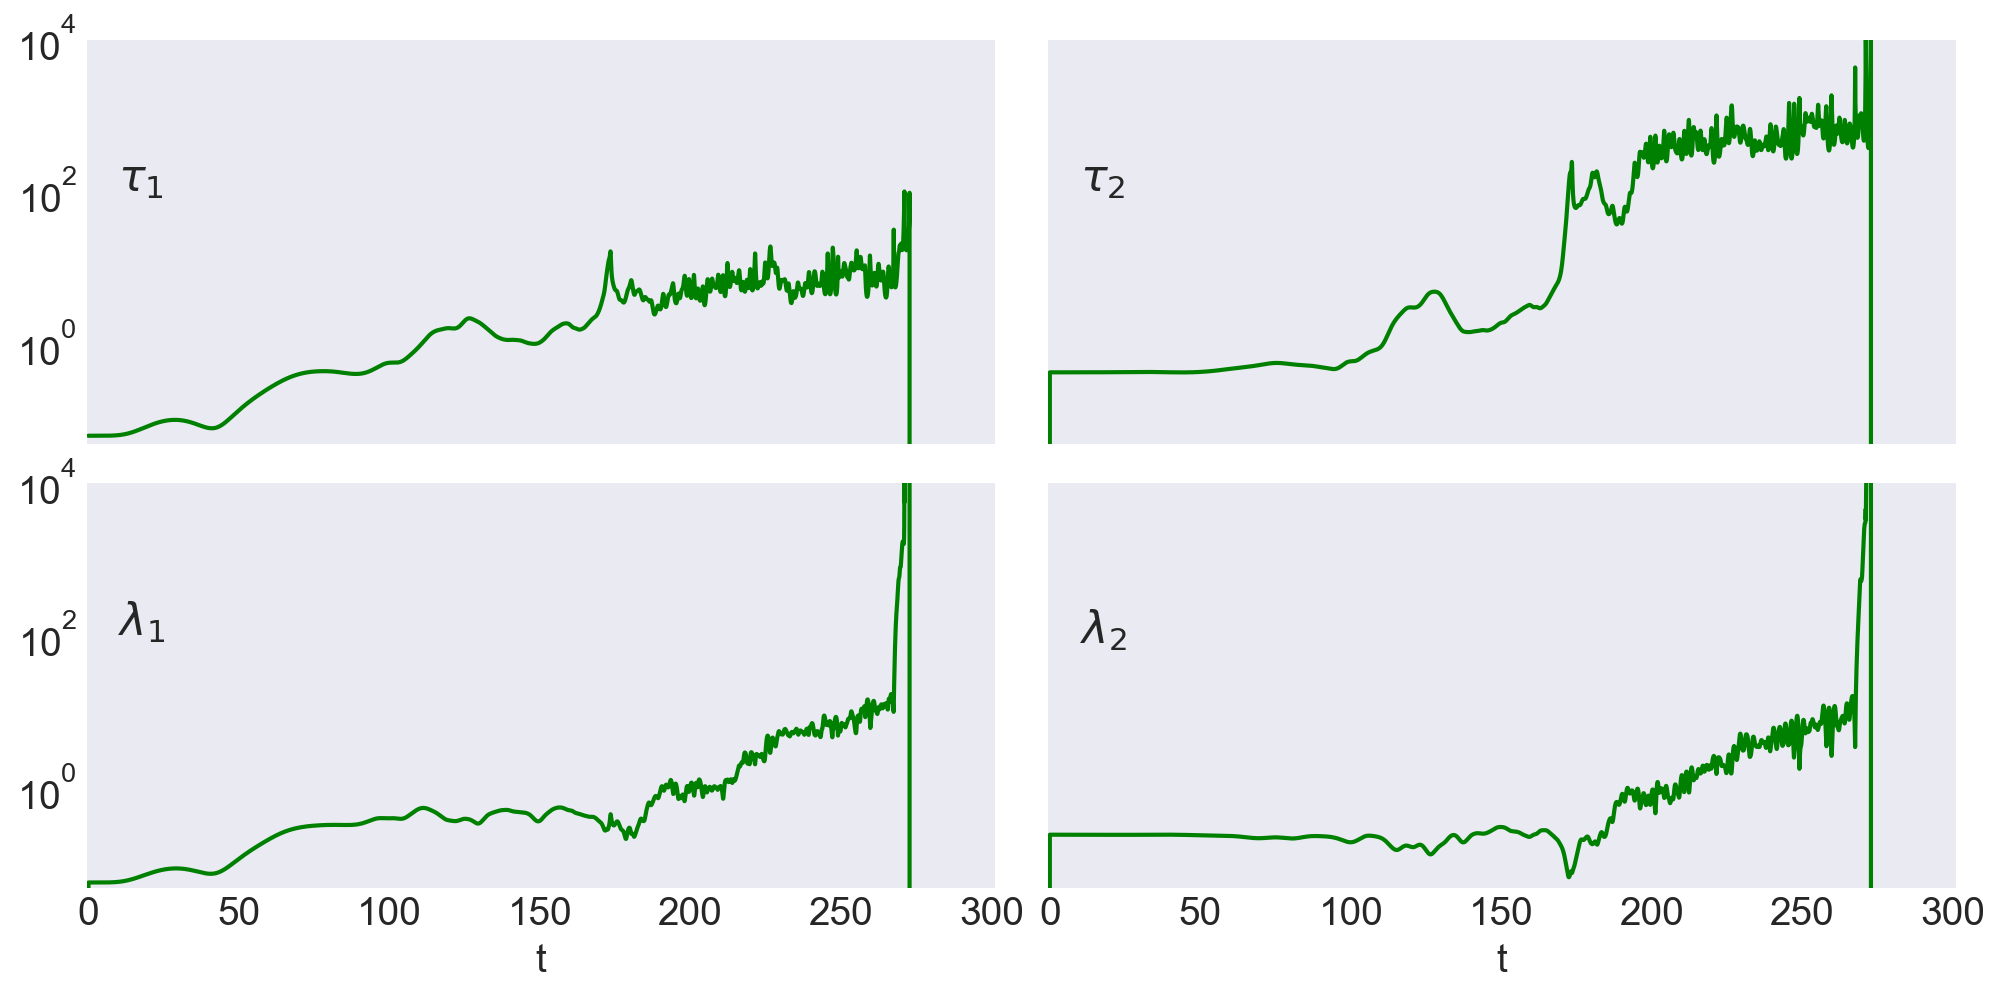
\includegraphics[width=\textwidth]{results/figures/miyagi/amplitude_norm_tdccsd.png} 
    \caption{Norm of the amplitudes over time in the 1D beryllium atom, computed 
        with TDCCSD. We see unreasonably high amplitude norms.
    }
    \label{fig:miyagi_tddccsd_amplitude}
\end{figure}

If we compute the norm of the amplitudes over the course of the simulation for 
the time-dependent coupled cluster singles doubles (TDCCSD) method, we get the 
result shown in \autoref{fig:miyagi_tddccsd_amplitude}. In essence, the amplitudes 
in any coupled cluster computation provides a linear combination of orbitals 
from the reference state $\ket{\Phi_0}$, in order to provide the best representation of the 
exact state $\ket{\Psi}$. For this reason one would not expect the norm of the 
amplitudes to be realtively low for an exact that is close to the reference state.
We encounter problems with the static orbitals because we are dealing with a system that
moves very far 
from its inital state. In \autoref{fig:miyagi_tddccsd_amplitude} we see
that the amplitudes stay within a reasonable magnitude for up to about halfway through 
the simulation, after which we see the method is struggling greatly to 
represent the current state with the basis it has been given. In figure 
\autoref{fig:miyagi_tdccsd_overlap}, a plot of the 
overlap of the current, time-dependent state with the initial ground state
helps to underline this point. The inset figure in \autoref{fig:miyagi_tdccsd_overlap}
shows the area of the figure with the highest value for the overlap, at a larger scale.
We see that the ground state probability reaches values of more than $300$, which is 
most definitely unreasonable, because a probability like this should always be between 
$0$ and $1$.

\begin{figure}
    \centering
    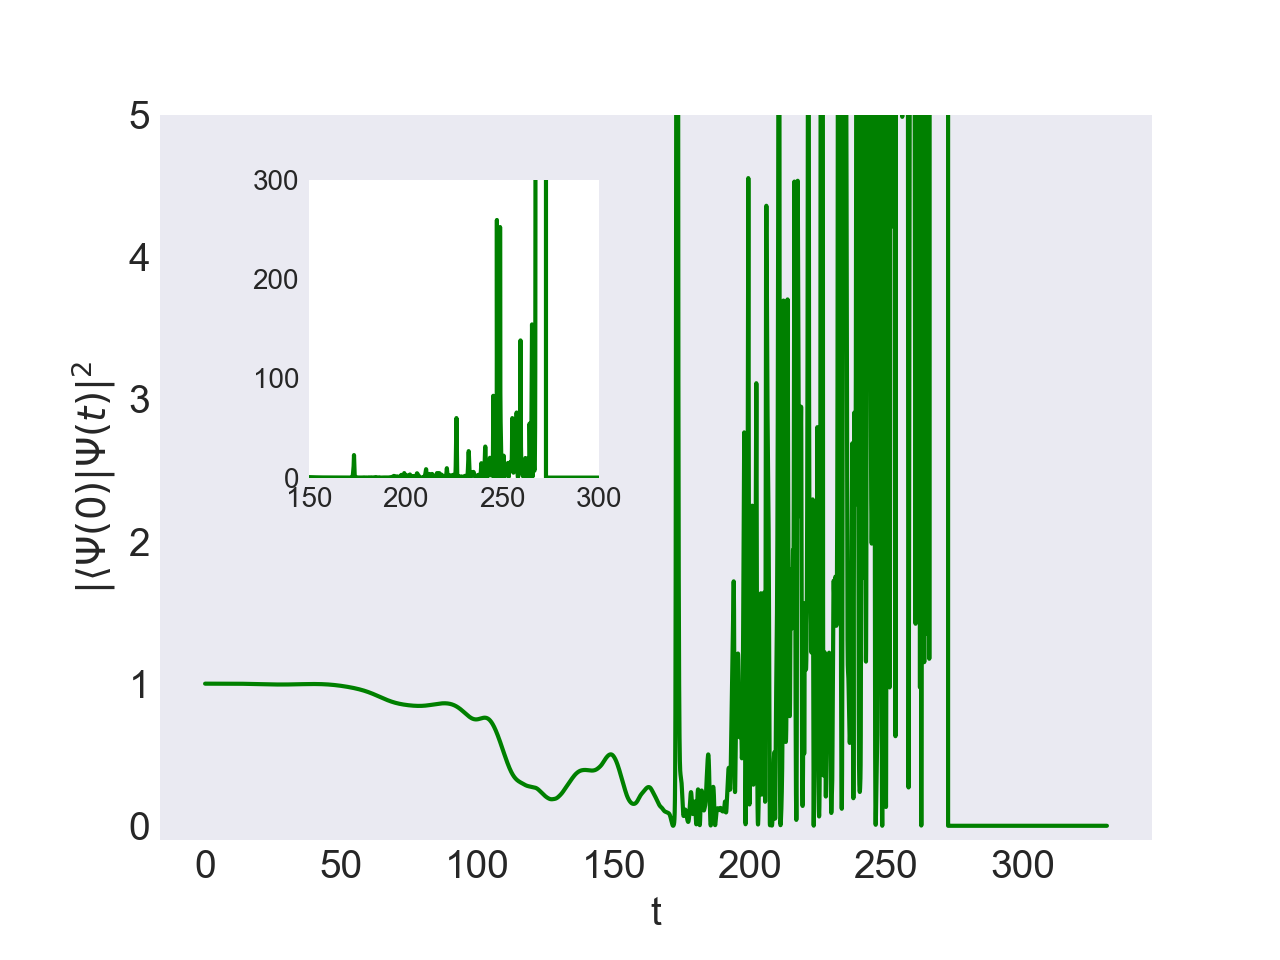
\includegraphics[width=0.75\textwidth]{results/figures/miyagi/overlap_tdccsd.png}
    \caption{Probability of being in the ground state over time 
        $|\braket{\Psi(0)}{\Psi(t)}|$ in the 1D beryllium atom, computed with TDCCSD. 
        We see impossibly unreasonable probabilities.
    }
    \label{fig:miyagi_tdccsd_overlap}
\end{figure}

It is difficult to draw a clear conclusion as to when the time-dependent coupled cluster 
method with static orbitals breaks down and is unfeasible for use. However, we can 
draw some broader, qualitative strokes towards a diagnosis of the problem. Any coupled 
cluster method is supposed to provide the best representation of a system's exact 
wavefunction by picking fitting parts of the basis set contained in the reference 
state for that system. If the exact wavefunction exists in a very different basis 
space than the reference state, it stands to reason that it is very difficult, if 
not impossible to find a mapping between the two. This problem stems from the foundations 
of the approximative nature of the coupled cluster method as it has a truncated basis set. 

\citeauthor{pedersen2019symplectic}\cite{pedersen2019symplectic} provide a similar 
deduction, highlighting there appears to be system-dependent upper limit for 
the strength of the external field. They underline the improvement in the computations 
by using a symplectic integrator instead of a standard fourth-order Runge-Kutta method.
We use the exact same integrator as the one \citeauthor{pedersen2019symplectic} outline.
\citeauthor{pedersen2019symplectic} argue that a large amplitude norm should make one 
question the validity of the result. It is difficult to gauge what constitutes a ``large''
amplitude norm, however.

Lastly with regards to the ionisation study from \citeauthor{miyagi2013time}\cite{miyagi2013time},
we would like to emphasise how well the orbital-adaptive time-dependent coupled cluster 
doubles (OATDCCD) method performs. OATDCCD manages to replicate the desired results 
to a significant degree, giving relatively high values for the entire grid 
of the particle density represented in \autoref{fig:miyagi_tdccsd_overlap}. This is 
normally interpreted as a free praticle because one would expect the wavefunction of 
a free particle to spread out in space as time progresses.